% This is part of Un soupçon de mathématique sans être agressif pour autant
% Copyright (c) 2012
%   Laurent Claessens, Pauline Klein
% See the file fdl-1.3.txt for copying conditions.

\newcommand{\comp}{{\ \ldots\ldots\ }} %
\newcommand{\exe}[1]{\par \smallskip %
  \fontfamily{cmss}\selectfont Exemple : \  \normalfont%
  \begin{minipage}[t]{0.8\linewidth}%
    \textit{#1}%
  \end{minipage} \par%
  \medskip
}

%\documentclass[french,a4paper,12pt]{book}
%\input{../Macros}
%\geometry{vmargin=40pt,hmargin=40pt}
%% -------------------------------
%% Repertoire de figures
%\graphicspath{{Cours_Statistiques/}}  
%% -------------------------------
%\input{Macros_Cours}
%
%\begin{document}
%
%
%
%
%\setlength{\baselineskip}{16pt}
%
%\setcounter{chapter}{5}
%%\setcounter{section}{2}
%%\setcounter{subsection}{1}
%
%\newcommand{\voc}[1]{\fontfamily{ppl}\selectfont #1\normalfont}
%\newcommand{\voc}[1]{\fontfamily{cmss}\selectfont #1\normalfont}

%\newcommand{\rmq}[1]{\par \medskip %
%  \fontfamily{cmss}\selectfont \noindent Remarque : \  \normalfont%
%  \begin{minipage}[t]{0.89\linewidth} 
%    #1 
%  \end{minipage} \par%
%  \medskip
%}
%}
%\newcommand{\para}[1]{\par \medskip%
%  \fontfamily{cmss}\selectfont \noindent #1 %
%  \normalfont %
%}
%\newcommand{\parag}[2]{\par \medskip %
%  \fontfamily{cmss}\selectfont \noindent #1 \  \normalfont%
%  \begin{minipage}[t]{0.84\linewidth} 
%    #2
%  \end{minipage} \par%
%  \medskip
%}
%\newcommand{\paragit}[2]{\par \medskip %
%  \fontfamily{cmss}\selectfont \noindent #1 \  \normalfont%
%  \begin{minipage}[t]{0.84\linewidth} 
%    \textit{#2}
%  \end{minipage} \par%
%  \medskip
%}
%
%\newcommand{\definition}[1]{\par \medskip %
%  \fontfamily{cmss}\selectfont \noindent Définition : \\[2pt] 
%  \normalfont%
%  \fbox{
%    \begin{minipage}[t]{0.95\linewidth} #1 \end{minipage} \par%
%    \medskip
%  }    \medskip
%}
%%\let\DEFINITION=\definition
%%\renewenvironment{definition}{\DEFINITION\bgroup}{\egroup}
%




% %%%%%%%%%%%%%%%%%%%%%%%%%%%%%%%%%%%%%%%%%%%%%
%    DEBUT DU COURS
% %%%%%%%%%%%%%%%%%%%%%%%%%%%%%%%%%%%%%%%%%%%%%


\chapter{Statistique descriptive}


Le rôle de la statistique descriptive est de présenter une masse de
données sous forme lisible, puis, si possible, de la résumer par
quelques nombres caractéristiques (moyenne, médiane, {\ldots} ).



% %%%%%%%%%%%%%%%%%%%%%%%%%%%%%%%%%%%%%%%%%%%%%
%    VOCABULAIRE
% %%%%%%%%%%%%%%%%%%%%%%%%%%%%%%%%%%%%%%%%%%%%%

\section{Vocabulaire}

\begin{enumerate}
    \item La \defe{population}{} désigne l'ensemble des personnes ou objets,
  aussi appelés individus, sur lesquels porte l'étude
  statistique.  
  \exe{Les élèves de la classe de 2\up{nde}B, les habitants d'un pays,
    les voitures produites en 2010, les employés d'une entreprise.}
\item On recueille alors des données concernant un \defe{caractère}{} sur
  les individus de cette population. Ce caractère peut prendre un
  certain nombre de \defe{valeurs}{}, numériques ou non.
  \exe{La taille des élèves de la classe, le salaire des employés, la
  couleur des voitures construites.}
\item Un caractère est dit \defe{quantitatif}{} lorsqu'il est possible de
  le mesurer en associant un nombre à chaque individu. Dans ce cas, le
  caractère quantitatif est aussi appelé \defe{variable}{}.
  \exe{L'âge, la taille, le nombre d'enfants dans une famille.}
  \begin{itemize}
      \item Un caractère quantitatif est dit \defe{continu}{} lorsque les
    nombres qui le mesurent peuvent prendre a priori toutes les
    valeurs d'un intervalle.
    \exe{La taille, un salaire, la durée de vie d'un baladeur.}
\item Le caractère est dit \defe{discret}{} dans le cas contraire.
    \exe{L'année de naissance, le nombre de frères et soeurs.}
  \end{itemize}
\item On appelle caractère \defe{qualitatif}{} tout caractère qui n'est
  pas quantitatif.
  \exe{La couleur des yeux, le chanteur préféré, le choix de la
    section de 1\up{ère}.} 
\end{enumerate}
Dans ce chapitre, on étudiera des séries statistiques dont le
caractère est \underline{quantitatif}.



\begin{minipage}[t]{1.0\linewidth}
\exe{Une revue présente un tableau donnant les prix
  en euros d'appareils photos numériques.}

\hspace{4.5em}
\begin{minipage}[t]{0.8\linewidth}
 

  {\centering
    \begin{tabular}[t]{|l|c|c|c|c|}
      \hline
      \textbf{Prix} & $[300;500[$ & $[500;700[$ & $[700;900[$ &
      $[900;1\,100[$ \\
      \hline
      \textbf{Effectif} & 14 & 8 & 3 & 1 \\
      \hline
    \end{tabular}
    \par}
  \bigskip

  \begin{itemize}
  \item Quelle est la population étudiée ? \\[1ex]
  \item Quel est le nombre d'individus de cette population ?\\[1ex]
  \item Quel est le caractère ? \\[1ex]
  \item Ce caractère est-il quantitatif ?
  \end{itemize}
  
\end{minipage}
\end{minipage}


%\vspace{0.5cm}



% %%%%%%%%%%%%%%%%%%%%%%%%%%%%%%%%%%%%%%%%%%%%%
%    PRESENTATION D'UNE SERIE
% %%%%%%%%%%%%%%%%%%%%%%%%%%%%%%%%%%%%%%%%%%%%%

\section{Présentation des éléments d'une série statistique}

\subsection{Effectifs. Effectifs cumulés croissants}

On donne souvent une série statistique par un tableau d'effectifs.

\exe{Dans un village, on recense le nombre d'enfants par foyer.}

\noindent
\textbf{Tableau 1}\\[-2ex]
\begin{tabular}[t]{|l|*{8}{>{\centering}p{1cm}<{}|}c}
  \cline{1-9}
  \textbf{Nombre d'enfants $x_i$} & 0 & 1 & 2 & 3 & 4 & 5 & 6 & 7 &\\
  \cline{1-9}
  \textbf{Effectif $n_i$} & 290 & 170 & 155 & 95 & 43 & 27 & 20 & 10 &\\
  \cline{1-9}
\end{tabular}
\medskip

On note généralement $N$ l'\defe{effectif total}{},
$N=n_1+n_2+n_3+{\ldots}+n_8$. 
\medskip

\textit{Ici, l'effectif total vaut :  \comp. }
\bigskip

Le \defe{mode}{} est la valeur ayant le plus grand effectif. Elle a un
intérêt si l'effectif de cette valeur est nettement plus grand que les
autres effectifs. Il peut y avoir plusieurs modes.
\medskip

\textit{Dans cet exemple, le mode est égal à \comp.}
\bigskip

A partir du tableau 1, on peut dresser le tableau des \defe{effectifs
cumulés croissants}{}.
\medskip

\noindent
\textbf{Tableau 2} \\[-2ex]
\begin{tabular}[t]{|l|*{8}{>{\centering}p{1cm}<{}|}c}
  \cline{1-9}
  \textbf{Nombre d'enfants $x\leq$} & 0 & 1 & 2 & 3 & 4 & 5 & 6 & 7 &\\
  \cline{1-9}
%   \textbf{Effectif $n_i$} & 290 & 170 & 155 & 95 & 43 & 27 & 20 & 10 &\\
%   \cline{1-9}
  \textbf{Effectif cumulé croissant} & 290 & 460 &  &  &  &
  &  &  &\\ 
  \cline{1-9}
\end{tabular}

\bigskip
\smallskip

%\paragraph{Interprétation :} 
%\begin{minipage}[t]{0.8\linewidth}
\noindent
Dans le tableau 1, on lit que \comp foyers ont 2 enfants. \\[1ex]
Dans le tableau 2, on lit que le nombre d'enfants est inférieur ou
égal à 2 dans \comp foyers.\\
% \end{minipage} \\

\begin{remark}
Le tableau des effectifs cumulés donne directement le nombre de
  foyers qui ont au plus $x_i$ enfants. \\
  Par exemple, pour $x_i=5$, il
  y a \comp foyers qui ont au plus 5 enfants.
\end{remark}


\medskip

\begin{remark}
Le tableau des effectifs cumulés permet également de repérer
  facilement la $n$-ième valeur donnée de la série triée par ordre
  croissant. \\
  Par exemple, le $750$\ieme{} foyer correspond à un foyer ayant
  \comp  enfants. 

    
\end{remark}


\vspace{1cm}

\subsection{Fréquences. Fréquences cumulées croissantes}

A partir des effectifs, on peut dresser le tableau des fréquences.

Par définition, la \defe{fréquence}{} d'une valeur du caractère $x_i$ est :
\[
\mbox{fréquence} 
= \frac{\mbox{effectif $n_i$ du caractère}}{\mbox{effectif total}}
\qquad
\mbox{soit} 
\qquad
f_i = \dfrac{n_i}{N}
\]
Ainsi, $f_1 = \dfrac{n_1}{N} = \dfrac{290}{810} \approx 0,36$.
\medskip

\noindent
\begin{tabular}[t]{|l|*{8}{>{\centering}p{1cm}<{}|}c}
  \cline{1-9}
  \textbf{Valeur $x_i$} & 0 & 1 & 2 & 3 & 4 & 5 & 6 & 7 &\\
  \cline{1-9}
  \textbf{Fréquence $f_i$} & 0,36 & 0,21 & 0,19 &  &  &
  &  &  &\\ 
  \cline{1-9}
\end{tabular}

\bigskip

\begin{remark}

  \begin{itemize}
  \item Une fréquence est toujours comprise entre 0 et 1. 
    \quad $0\leq f_i\leq 1$. \\[-2ex]
  \item La somme des fréquences est toujours égale à 1. \
    \quad $f_1+f_2+{\ldots}+f_8 =  1$.
  \end{itemize}


    
\end{remark}

\bigskip

A partir du tableau des fréquences, on peut dresser le tableau des
\defe{fréquences cumulées croissantes}{}, en ajoutant à chaque fréquence
la somme des fréquences précédentes.

\medskip

\noindent
\begin{tabular}[t]{|l|*{7}{>{\centering}p{1cm}<{}|}c}
  \cline{1-8}
  \textbf{Valeur $x_i$} & 0 & 1 & 2 & 3 & 4 & \ldots & 7 &\\
  \cline{1-8}
  \textbf{Fréquence $f_i$} & 0,36 & 0,21 & 0,19 & 0,12 &  & \ldots &  &\\ 
  \cline{1-8}
  \textbf{Fréquence cumulée croissante} & 0,36 & 0,57 & 0,76 &  &  &
  \ldots  & 1 &\\ 
  \cline{1-8}
\end{tabular}

\bigskip

A partir du tableau des fréquences cumulées, on lit que \comp \% des
foyers ont moins de 3 enfants, et \comp \% des foyers ont moins de 4 enfants.

\bigskip

\vspace{1cm}


\subsection{Représentation en classes}

Lorsque les valeurs étudiées sont en très grand nombre, on peut les
regrouper dans des intervalles de la forme $[a;b[$ appelés
    \defe{classes}{}. 

    L'\defe{amplitude}{} de la classe est $b-a$, c'est l'écart entre la plus
grande et la plus petite valeur de la classe.

Le \defe{centre}{} de la classe est la moyenne $\dfrac{a+b}2$.

La \defe{classe modale}{} est la classe qui a le plus grand effectif. 

\medskip

\exe{Le tableau ci-dessous donne la répartition des masses de
  nouveaux-nés dans un hôpital, de 2,5 $kg$ à 4,5 $kg$.
}
\smallskip

\hspace{4.5em}
\begin{minipage}[t]{0.8\linewidth}
  \begin{tabular}[t]{|l|c|c|c|c|}
    \hline
    \textbf{Masse en kg} & $[2,\!5\,;3[$ & $[3\,;3,\!5[$ & $[3,\!5\,;4[$ &
    $[4\,;4,\!5[$ \\
    \hline
    \textbf{Effectif} & 15 & 32 & 40 & 13 \\
    \hline
  \end{tabular}
  \bigskip
  
  \textit{L'effectif total est égal à \comp.} \\[1ex]
  \textit{L'amplitude des classes est égale à \comp.} \\[1ex]
  \textit{Le centre de la deuxième classe est \comp.} \\[1ex]
  \textit{La classe modale est \comp.}

\end{minipage}



%\vspace{1cm}








\clearpage


% %%%%%%%%%%%%%%%%%%%%%%%%%%%%%%%%%%%%%%%%%%%%%
%    VALEURS CARACTERISTIQUES
% %%%%%%%%%%%%%%%%%%%%%%%%%%%%%%%%%%%%%%%%%%%%%

\renewcommand{\exe}[1]{\par %\smallskip %
  \noindent%
  \fontfamily{cmss}\selectfont Exemple : \  \normalfont%
  \begin{minipage}[t]{0.85\linewidth}%
    \textit{#1}%
  \end{minipage} \par%
  \medskip
}

\section{Etude d'une série statistique : grandeurs caractéristiques}

On considère une série statistique dont les valeurs du caractère sont
$x_1$, $x_2$, {\ldots}, $x_p$, et les effectifs correspondants :
$n_1$, $n_2$, {\ldots}, $n_p$.

%\bigskip
%\medskip


\subsection{Moyenne}

\begin{definition}
    La \defe{moyenne}{} de la série statistique des $(x_i;n_i)$ est le
  nombre, noté $\overline{x}$, défini par
  \[
  \overline{x} =
  \frac{n_1x_1+n_2x_2+{\ldots}+n_px_p}{N} 
  \]
  où $N = n_1+n_2+{\ldots}+n_p$ est l'effectif total.

    
\end{definition}

\bigskip


\exe{On reprend le tableau 1 donnant le nombre d'enfants par foyer
  dans un village. Dans ce village, le nombre moyen d'enfants par
  foyer est  
\begin{align*}
  \overline{x} = {} & 
  \frac{290\times0+170\times1+155\times2+95\times
    3+43\times 4+27\times 5+20\times 6+10\times 7}{810}
  \\[1ex]
  \overline{x} \approx {} & 1,6
\end{align*}
}
\medskip

\begin{remark}
On peut aussi calculer $\overline{x}$ en utilisant les fréquences
  $f_i$ : \\[1ex]
  $ \overline{x} = f_1 x_1 + f_2x_2+{\ldots}+f_px_p $. 

    
\end{remark}

\bigskip



\subsection{Médiane}

\begin{definition}
    La \defe{médiane}{}, notée $M_e$, d'une série statistique est un
  nombre qui partage la population en deux parties :
  \begin{enumerate}
  \item 50 \% au moins des individus ont une valeur du caractère
    inférieure ou égale à $M_e$ ;
  \item 50 \% au moins des individus ont une valeur du caractère
    supérieure ou égale à $M_e$.
  \end{enumerate}  

    
\end{definition}


\paragraph{En pratique :}On range les $N$ valeurs de la série par ordre
  croissant, chacune étant répétée autant de fois que son effectif.


\begin{enumerate}
\item Si $N$ est impair, la médiane est la valeur centrale de la série ;
\item Si $N$ est pair, la médiane est la demi-somme des deux valeurs
  centrales de la série.
\end{enumerate}

%\bigskip
\medskip

\begin{example}
\begin{itemize}
\item Pour une série de 7 valeurs \underline{rangées par ordre
    croissant}, la médiane est \comp \comp \\[-4ex]
\item Si la série comporte 12 valeurs, la médiane est \comp \comp
  \comp \\[-1ex]
\item Si la série comporte 6 valeurs, la médiane est \comp \comp
  \comp \\[-1ex]
\item Si la série comporte 25 valeurs, la médiane est \comp \comp
  \comp \\[-1ex]
\item Si la série comporte 15 valeurs, la médiane est \comp \comp \comp
\end{itemize}
    
\end{example}



\paragraph{Application :}Dans chaque cas, déterminer la médiane de la
  série.\\
  Conseil : on commencera par trier les valeurs de la série par ordre
  croissant, et on donnera l'effectif total.


\begin{enumerate}
\item 5 ; 10 ; 17 ; 12 ; 6 
\item 1\,000 ; 1\,000 ; 1\,200 ; 1\,200 ; 1\,200 ; 1\,500 ; 1\,500 ;
  2\,000 ; 2\,500 ; 3\,100 
\item 5 ; 1 ; 2 ; 9 ; 4 ; 5 ; 7 ; 5 ; 9 ; 5 ; 6 ; 7 ; 8 ; 9 ; 2 ; 9 ;
  6 ; 5 ; 9 ; 3 
\end{enumerate}

\begin{remark}
La médiane ne dépend pas des valeurs extrêmes.

    
\end{remark}



\bigskip


\subsection{Quartiles}

\begin{definition}
  On considère une liste de $N$ valeurs, \underline{triées par ordre
    croissant}. 
  \begin{enumerate}
      \item Le \defe{premier quartile}{} $Q_1$ est la plus petite valeur de
    la liste telle qu'au moins un quart des valeurs de la liste sont
    inférieures ou égales à $Q_1$.
\item Le \defe{troisième quartile}{} $Q_3$ est la plus petite valeur de
    la liste telle qu'au moins les trois quarts des valeurs de la
    liste sont inférieures ou égales à $Q_3$.
  \end{enumerate}

    
\end{definition}

\bigskip

\paragraph{En pratique :}
  Pour le calcul de $Q_1$, on calcule $\dfrac{N}4$, puis on détermine
  le premier entier $p$ supérieur ou égal à $\dfrac{N}4$. Cet entier
  $p$ donne le rang de $Q_1$. \\
  Pour le calcul de $Q_3$, on fait de même en remplaçant $\dfrac{N}4$
  par $\dfrac{3N}4$. 


\bigskip


\exe{%
  \vspace{-4ex}
  \begin{enumerate}
  \item Pour $N=15$, on a \ $\dfrac{N}4 = 3,75$, donc $Q_1$ est la
    \comp\ieme{} valeur de la série (lorsqu'elle est rangée par ordre
    croissant). \\[1ex]
    De plus, \comp\comp, donc $Q_3$ est la \comp \up{e} valeur de la
    série. \\
  \item Pour $N=18$, $Q_1$ est la \comp\up{e} valeur, et $Q_3$ est la
    \comp\up{e} valeur de la série.
\end{enumerate}
}

\bigskip

%\clearpage

\paragraph{Application :}Déterminer le premier et le troisième quartile
  de chaque série.

\begin{enumerate}
\item 1\,000 ; 1\,000 ; 1\,200 ; 1\,200 ; 1\,200 ; 1\,500 ; 1\,500 ;
  2\,000 ; 2\,500 ; 3\,100 
\item  5 ; 1 ; 2 ; 9 ; 4 ; 5 ; 7 ; 5 ; 9 ; 5 ; 6 ; 7 ; 8 ; 9 ; 2 ; 9 ;
  6 ; 5 ; 9 ; 3
\end{enumerate}


\bigskip



\subsection{Mesures de dispersion}

\medskip

\begin{enumerate}
    \item L'\defe{étendue}{} d'une série statistique est la différence entre
  la plus grande et la plus petite valeur.
\item L'\defe{écart interquartile}{} est égal à la différence $Q_3-Q_1$.
\end{enumerate}

\bigskip

\exe{Pour la série  1\,000 ; 1\,000 ; 1\,200 ; 1\,200 ; 1\,200 ; 1\,500 ; 1\,500 ;
  2\,000 ; 2\,500 ; 3\,100 ; étudiée ci-dessus, \\[-2ex]
  \begin{itemize}
  \item l'étendue vaut \comp \\[-1ex]
  \item l'écart interquartile est égal à \comp.
  \end{itemize}
}

\bigskip


\subsection{Lecture des grandeurs caractéristiques à l'aide des
  effectifs cumulés croissants}

\noindent
\begin{tabular}[t]{|l|*{11}{>{\centering}p{0.8cm}<{}|}c}
  \cline{1-12}
  \textbf{Valeur} & 73 & 74 & 75 & 76 & 77 & 78 & 79 & 80 & 81 &
  82 & 83 &\\
  \cline{1-12}
  \textbf{Effectif} & 2 & 4 & 3 & 7 & 9 & 6 & 8 & 3 & 4 & 2 & 2 &\\ 
  \cline{1-12}
  \textbf{Eff. cum. cr.} & 2 & 6 & 9 & 16 & 25 & 31 & 39 &
  42 & 46 & 48 & 50 &\\ 
  \cline{1-12}
%   \textbf{F. c. c.} & 0,04 & 0,12 & 0,18 & 0,32 & 0,50 & 0,62 & 0,78 &
%   0,84 & 0,92 & 0,96 & 1 &\\ 
%   \cline{1-12}
\end{tabular}

\bigskip

\exe{Dans la série représentée par le tableau ci-dessus, l'effectif
  total est égal à 50.
  \begin{itemize}
  \item Le premier quartile est la 13\up{e} valeur.
  \item La médiane est la moyenne entre la 25\up{e} et la 26\up{e} valeurs.
  \item Le troisième quartile est la 38\up{e} valeur.
  \end{itemize}
\smallskip
A l'aide de la ligne des effectifs cumulés, donner :
\[ 
Q_1 = \comp , \qquad M_e = \comp , \qquad Q_3 = \comp 
\]
}

\bigskip
%\clearpage

\subsection{Lecture des quartiles à l'aide des fréquences cumulées croissantes}

Dans le tableau des fréquences cumulées croissantes :
\begin{itemize}
\item le premier quartile $Q_1$ est la première valeur de la série
  pour laquelle la fréquence cumulée croissante $0,25$ est atteinte ou
  dépassée ;
\item le troisième quartile $Q_3$ est la première valeur de la série
  pour laquelle la fréquence cumulée croissante $0,75$ est atteinte ou
  dépassée.
\end{itemize}

\medskip

\exe{}
\vspace{-1em}
\noindent
\begin{tabular}[t]{|l|*{11}{>{\centering}p{0.8cm}<{}|}c}
  \cline{1-12}
  \textbf{Valeur} & 73 & 74 & 75 & 76 & 77 & 78 & 79 & 80 & 81 &
  82 & 83 &\\
%  \cline{1-12}
%  \textbf{Effectif} & 2 & 4 & 2 & 7 & 9 & 6 & 8 & 3 & 4 & 2 & 2 &\\ 
%   \cline{1-12}
%   \textbf{Effectif cumulé} & 2 & 6 & 9 & 16 & 25 & 31 & 39 &
%   42 & 46 & 48 & 50 &\\ 
  \cline{1-12}
  \textbf{Freq. cum. cr.} & 0,04 & 0,12 & 0,18 & 0,32 & 0,50 & 0,62 & 0,78 &
  0,84 & 0,92 & 0,96 & 1 &\\ 
  \cline{1-12}
\end{tabular}

\smallskip

Le premier quartile vaut \ $Q_1=\comp$. Le troisième quartile vaut \ $Q_3=\comp$. 



\clearpage


% %%%%%%%%%%%%%%%%%%%%%%%%%%%%%%%%%%%%%%%%%%%%%
%    REPRESENTATION GRAPHIQUE
% %%%%%%%%%%%%%%%%%%%%%%%%%%%%%%%%%%%%%%%%%%%%%

\section{Représentation graphique d'une série statistique}


\begin{multicols}{2}
\subsection{Nuage de points}
  \begin{itemize}
  \item En abscisses, les valeurs du caractère.
  \item En ordonnées, les effectifs (ou les fréquences)
  \end{itemize}
  \columnbreak
  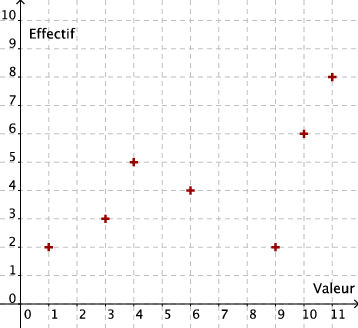
\includegraphics[width=5cm]{Stats_Fig4_Nuage}      
\end{multicols}



\subsection{Diagramme en bâtons, ou diagramme en barres}


\begin{multicols}{2}
\begin{itemize}
\item Pour des caractères qualitatifs.
\item L'abscisse représente les valeurs.
\item La hauteur du bâton est proportionnelle à l'effectif (ou à la fréquence).
\end{itemize}

\medskip
\exe{V{\oe}u d'orientation des élèves d'une classe de seconde}
\columnbreak
  \begin{center}
    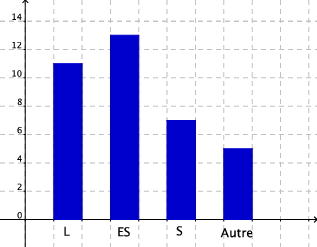
\includegraphics[width=6cm]{Stats_Fig4_DiagBaton}
  \end{center}    
\end{multicols}




\subsection{Histogramme}

\begin{itemize}
\item Pour des données rassemblées en classes
\item L'\textbf{aire} du rectangle est proportionnelle à l'effectif (ou à la
fréquence). 
\end{itemize}

\begin{multicols}{2}
  \begin{center}
    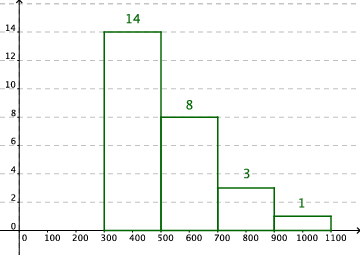
\includegraphics[width=6cm]{Stats_Fig4_HistPC}
    Histogramme à pas constant \\
    (classes de même amplitude)     
  \end{center}

  \columnbreak

  \begin{center}
    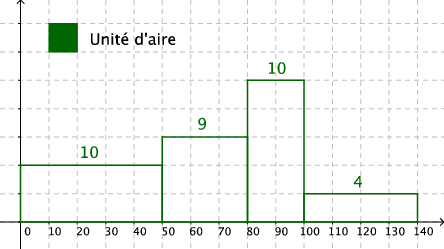
\includegraphics[width=6cm]{Stats_Fig4_HistPNC}
    Histogramme à pas non constant \\
    (classes d'amplitudes différentes)
  \end{center}
  
\end{multicols}


%\medskip


\subsection{Diagramme circulaire}

\begin{multicols}{2}
  \begin{itemize}
  \item L'angle au centre du secteur circulaire est proportionnel à l'effectif
    de chaque valeur.
  \end{itemize}
  
  \medskip
  
  \exe{Production de fromages en France, en milliers de tonnes
  }
  \columnbreak
  \begin{minipage}{1.0\linewidth}
    \vspace{-2em}
    \begin{center}
      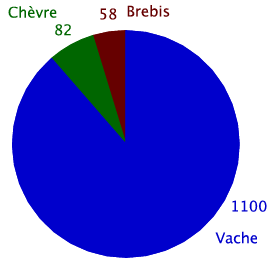
\includegraphics[width=5cm]{Stats_Fig4_DiagCirc}
    \end{center}    
  \end{minipage}
\end{multicols}



\subsection{Diagramme des effectifs/fréquences cumulé(e)s croissant(e)s}

\begin{multicols}{2}
  \begin{center}
    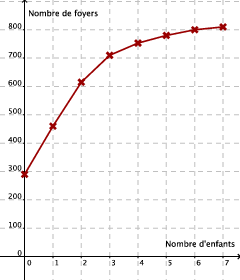
\includegraphics[width=6cm]{Stats_Fig4_DiagEffCum}
    
    Diagramme des effectifs cumulés croissants    
  \end{center}

  \columnbreak
  \begin{center}
    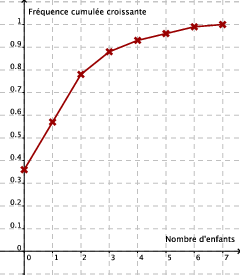
\includegraphics[width=6cm]{Stats_Fig4_DiagFreqCum}

    Diagramme des fréquences cumulées croissantes
  \end{center}
\end{multicols}



\subsection{Diagramme en boîte, ou diagramme à moustaches}

\begin{itemize}
\item Pour des séries ayant un grand nombre de valeurs
\item Basé sur les quartiles et la médiane
\end{itemize}

\begin{center}
  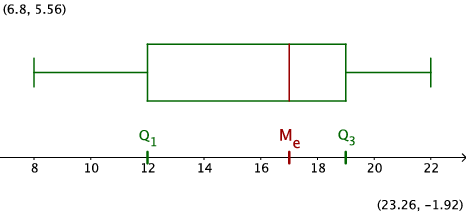
\includegraphics[width=7cm]{Stats_Fig4_DiagBoite}  
\end{center}


% %%%%%%%%%%%%%%%%%%%%%%%%%%%%%%%%%%%%%%%%%%%%%
%    VALEURS CARACTERISTIQUES
% %%%%%%%%%%%%%%%%%%%%%%%%%%%%%%%%%%%%%%%%%%%%%

\section{Etude d'une série statistique : grandeurs caractéristiques}

On considère une série statistique dont les valeurs du caractère sont
$x_1$, $x_2$, {\ldots}, $x_p$, et les effectifs correspondants :
$n_1$, $n_2$, {\ldots}, $n_p$.


\subsection{Moyenne}

\begin{definition}
    La \defe{moyenne}{} de la série statistique des $(x_i;n_i)$ est le
  nombre, noté $\overline{x}$, défini par
  \[
  \overline{x} =
  \frac{n_1x_1+n_2x_2+{\ldots}+n_px_p}{N} 
  \]
  où $N = n_1+n_2+{\ldots}+n_p$ est l'effectif total.

    
\end{definition}

\bigskip


\exe{On reprend le tableau 1 donnant le nombre d'enfants par foyer
  dans un village. Dans ce village, le nombre moyen d'enfants par
  foyer est  
\begin{align*}
  \overline{x} = {} & 
  \frac{290\times0+170\times1+155\times2+95\times
    3+43\times 4+27\times 5+20\times 6+10\times 7}{810}
  \\[1ex]
  \overline{x} \approx {} & 1,6
\end{align*}
}
\medskip

\begin{remark}
On peut aussi calculer $\overline{x}$ en utilisant les fréquences
  $f_i$ : \\[1ex]
  $ \overline{x} = f_1 x_1 + f_2x_2+{\ldots}+f_px_p $. 

    
\end{remark}

\bigskip



\subsection{Médiane}

\begin{definition}
    La \defe{médiane}{}, notée $M_e$, d'une série statistique est un
  nombre qui partage la population en deux parties :
  \begin{enumerate}
  \item 50 \% au moins des individus ont une valeur du caractère
    inférieure ou égale à $M_e$ ;
  \item 50 \% au moins des individus ont une valeur du caractère
    supérieure ou égale à $M_e$.
  \end{enumerate}  

    
\end{definition}

\bigskip

\paragraph{En pratique :}On range les $N$ valeurs de la série par ordre
  croissant, chacune étant répétée autant de fois que son effectif.


\begin{enumerate}
\item Si $N$ est impair, la médiane est la valeur centrale de la série ;
\item Si $N$ est pair, la médiane est la demi-somme des deux valeurs
  centrales de la série.
\end{enumerate}

\medskip

\begin{example}
\begin{itemize}
\item Pour une série de 7 valeurs \underline{rangées par ordre
    croissant}, la médiane est \comp \comp \\[-4ex]
\item Si la série comporte 12 valeurs, la médiane est \comp \comp
  \comp \\[-1ex]
\item Si la série comporte 6 valeurs, la médiane est \comp \comp
  \comp \\[-1ex]
\item Si la série comporte 25 valeurs, la médiane est \comp \comp
  \comp \\[-1ex]
\item Si la série comporte 15 valeurs, la médiane est \comp \comp \comp
\end{itemize}

    
\end{example}


\paragraph{Application :}Dans chaque cas, déterminer la médiane de la
  série.\\
  Conseil : on commencera par trier les valeurs de la série par ordre
  croissant, et on donnera l'effectif total.

\smallskip

\begin{enumerate}
\item 5 ; 10 ; 17 ; 12 ; 6 
\item 1\,000 ; 1\,000 ; 1\,200 ; 1\,200 ; 1\,200 ; 1\,500 ; 1\,500 ;
  2\,000 ; 2\,500 ; 3\,100 
\item 5 ; 1 ; 2 ; 9 ; 4 ; 5 ; 7 ; 5 ; 9 ; 5 ; 6 ; 7 ; 8 ; 9 ; 2 ; 9 ;
  6 ; 5 ; 9 ; 3 
\end{enumerate}

\begin{remark}
La médiane ne dépend pas des valeurs extrêmes.

    
\end{remark}



\bigskip


\subsection{Quartiles}

\begin{definition}
  On considère une liste de $N$ valeurs, \underline{triées par ordre
    croissant}. 
  \begin{enumerate}[\textbullet]
      \item Le \defe{premier quartile}{} $Q_1$ est la plus petite valeur de
    la liste telle qu'au moins un quart des valeurs de la liste sont
    inférieures ou égales à $Q_1$.
\item Le \defe{troisième quartile}{} $Q_3$ est la plus petite valeur de
    la liste telle qu'au moins les trois quarts des valeurs de la
    liste sont inférieures ou égales à $Q_3$.
  \end{enumerate}

    
\end{definition}

\bigskip

\paragraph{En pratique :}
  Pour le calcul de $Q_1$, on calcule $\dfrac{N}4$, puis on détermine
  le premier entier $p$ supérieur ou égal à $\dfrac{N}4$. Cet entier
  $p$ donne le rang de $Q_1$. \\
  Pour le calcul de $Q_3$, on fait de même en remplaçant $\dfrac{N}4$
  par $\dfrac{3N}4$. 


\bigskip


\exe{%
  \vspace{-4ex}
  \begin{enumerate}
  \item Pour $N=15$, on a \ $\dfrac{N}4 = 3,75$, donc $Q_1$ est la
    \comp\ieme{} valeur de la série (lorsqu'elle est rangée par ordre
    croissant). 
    De plus, \comp\comp, donc $Q_3$ est la \comp \up{e} valeur de la
    série. \\
  \item Pour $N=18$, $Q_1$ est la \comp\up{e} valeur, et $Q_3$ est la
    \comp\up{e} valeur de la série.
\end{enumerate}
}

\bigskip


\paragraph{Application :}Déterminer le premier et le troisième quartile
  de chaque série.

\begin{enumerate}
\item 1\,000 ; 1\,000 ; 1\,200 ; 1\,200 ; 1\,200 ; 1\,500 ; 1\,500 ;
  2\,000 ; 2\,500 ; 3\,100 
\item  5 ; 1 ; 2 ; 9 ; 4 ; 5 ; 7 ; 5 ; 9 ; 5 ; 6 ; 7 ; 8 ; 9 ; 2 ; 9 ;
  6 ; 5 ; 9 ; 3
\end{enumerate}


\bigskip



\subsection{Mesures de dispersion}

\medskip

\begin{enumerate}
    \item L'\defe{étendue}{} d'une série statistique est la différence entre
  la plus grande et la plus petite valeur.
\item L'\defe{écart interquartile}{} est égal à la différence $Q_3-Q_1$.
\end{enumerate}

\bigskip

\exe{Pour la série  1\,000 ; 1\,000 ; 1\,200 ; 1\,200 ; 1\,200 ; 1\,500 ; 1\,500 ;
  2\,000 ; 2\,500 ; 3\,100 ; étudiée ci-dessus, \\[-2ex]
  \begin{itemize}
  \item l'étendue vaut \comp \\[-1ex]
  \item l'écart interquartile est égal à \comp.
  \end{itemize}
}

\bigskip


\subsection{Lecture des grandeurs caractéristiques à l'aide des
  effectifs cumulés croissants}

\noindent
\begin{tabular}[t]{|l|*{11}{>{\centering}p{0.8cm}<{}|}c}
  \cline{1-12}
  \textbf{Valeur} & 73 & 74 & 75 & 76 & 77 & 78 & 79 & 80 & 81 &
  82 & 83 &\\
  \cline{1-12}
  \textbf{Effectif} & 2 & 4 & 2 & 7 & 9 & 6 & 8 & 3 & 4 & 2 & 2 &\\ 
  \cline{1-12}
  \textbf{Eff. cum. cr.} & 2 & 6 & 9 & 16 & 25 & 31 & 39 &
  42 & 46 & 48 & 50 &\\ 
  \cline{1-12}
\end{tabular}

\bigskip

\exe{Dans la série représentée par le tableau ci-dessus, l'effectif
  total est égal à 50.
  \begin{itemize}
  \item Le premier quartile est la 13\up{e} valeur.
  \item La médiane est la moyenne entre la 25\up{e} et la 26\up{e} valeurs.
  \item Le troisième quartile est la 38\up{e} valeur.
  \end{itemize}
\smallskip
A l'aide de la ligne des effectifs cumulés, donner :
\[ 
Q_1 = \comp , \qquad M_e = \comp , \qquad Q_3 = \comp 
\]
}

\bigskip


\subsection{Lecture des quartiles à l'aide des fréquences cumulées croissantes}

Dans le tableau des fréquences cumulées croissantes :
\begin{itemize}
\item le premier quartile $Q_1$ est la première valeur de la série
  pour laquelle la fréquence cumulée croissante $0,25$ est atteinte ou
  dépassée ;
\item le troisième quartile $Q_3$ est la première valeur de la série
  pour laquelle la fréquence cumulée croissante $0,75$ est atteinte ou
  dépassée.
\end{itemize}

\medskip

\exe{}
\vspace{-1em}
\noindent
\begin{tabular}[t]{|l|*{11}{>{\centering}p{0.8cm}<{}|}c}
  \cline{1-12}
  \textbf{Valeur} & 73 & 74 & 75 & 76 & 77 & 78 & 79 & 80 & 81 &
  82 & 83 &\\
  \cline{1-12}
  \textbf{Freq. cum. cr.} & 0,04 & 0,12 & 0,18 & 0,32 & 0,50 & 0,62 & 0,78 &
  0,84 & 0,92 & 0,96 & 1 &\\ 
  \cline{1-12}
\end{tabular}

\smallskip

Le premier quartile vaut \ $Q_1=\comp$. \\[1ex]  Le troisième quartile vaut \ $Q_3=\comp$. }



\clearpage


% %%%%%%%%%%%%%%%%%%%%%%%%%%%%%%%%%%%%%%%%%%%%%
%    REPRESENTATION GRAPHIQUE
% %%%%%%%%%%%%%%%%%%%%%%%%%%%%%%%%%%%%%%%%%%%%%

\section{Représentation graphique d'une série statistique}


\begin{multicols}{2}
\subsection{Nuage de points}
  \begin{itemize}
  \item En abscisses, les valeurs du caractère.
  \item En ordonnées, les effectifs (ou les fréquences)
  \end{itemize}
  \columnbreak
  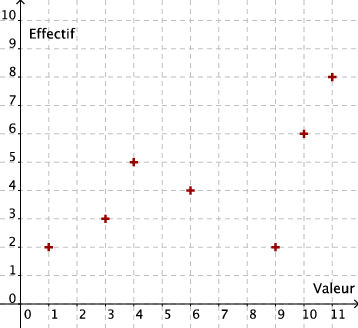
\includegraphics[width=5cm]{Stats_Fig4_Nuage}      
\end{multicols}



\subsection{Diagramme en bâtons, ou diagramme en barres}


\begin{multicols}{2}
\begin{itemize}
\item Pour des caractères qualitatifs.
\item L'abscisse représente les valeurs.
\item La hauteur du bâton est proportionnelle à l'effectif (ou à la fréquence).
\end{itemize}

\medskip
\exe{V{\oe}u d'orientation des élèves d'une classe de seconde}
\columnbreak
  \begin{center}
    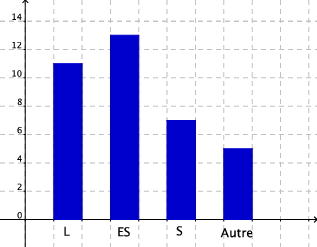
\includegraphics[width=6cm]{Stats_Fig4_DiagBaton}
  \end{center}    
\end{multicols}




\subsection{Histogramme}

\begin{itemize}
\item Pour des données rassemblées en classes
\item L'\textbf{aire} du rectangle est proportionnelle à l'effectif (ou à la
fréquence). 
\end{itemize}

\begin{multicols}{2}
  \begin{center}
    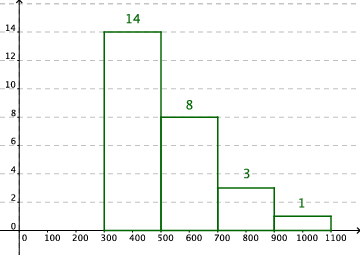
\includegraphics[width=6cm]{Stats_Fig4_HistPC}
    Histogramme à pas constant \\
    (classes de même amplitude)     
  \end{center}

  \columnbreak

  \begin{center}
    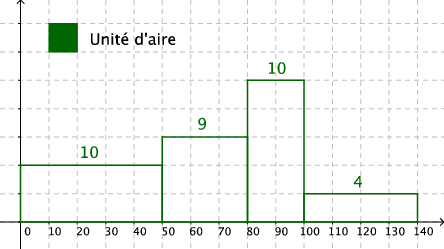
\includegraphics[width=6cm]{Stats_Fig4_HistPNC}
    Histogramme à pas non constant \\
    (classes d'amplitudes différentes)
  \end{center}
  
\end{multicols}



\subsection{Diagramme circulaire}

\begin{multicols}{2}
  \begin{itemize}
  \item L'angle au centre du secteur circulaire est proportionnel à l'effectif
    de chaque valeur.
  \end{itemize}
  
  \medskip
  
  \exe{Production de fromages en France, en milliers de tonnes
  }
  \columnbreak
  \begin{minipage}{1.0\linewidth}
    \vspace{-2em}
    \begin{center}
      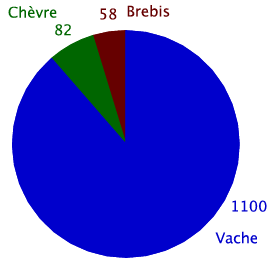
\includegraphics[width=5cm]{Stats_Fig4_DiagCirc}
    \end{center}    
  \end{minipage}
\end{multicols}



\subsection{Diagramme des effectifs/fréquences cumulé(e)s croissant(e)s}

\begin{multicols}{2}
  \begin{center}
    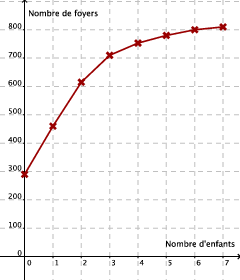
\includegraphics[width=6cm]{Stats_Fig4_DiagEffCum}
    
    Diagramme des effectifs cumulés croissants    
  \end{center}

  \columnbreak
  \begin{center}
    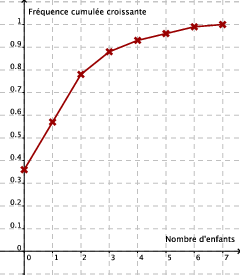
\includegraphics[width=6cm]{Stats_Fig4_DiagFreqCum}

    Diagramme des fréquences cumulées croissantes
  \end{center}
\end{multicols}

\subsection{Diagramme en boîte, ou diagramme à moustaches}

\begin{itemize}
\item Pour des séries ayant un grand nombre de valeurs
\item Basé sur les quartiles et la médiane
\end{itemize}

\begin{center}
  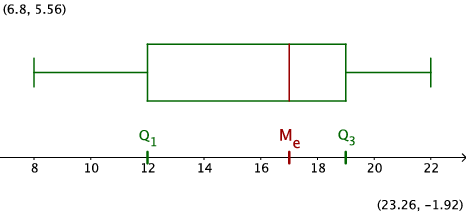
\includegraphics[width=7cm]{Stats_Fig4_DiagBoite}  
\end{center}



